\documentclass[10pt,twocolumn]{article}
\usepackage[a4paper,top=0.7in,bottom=0.75in,left=0.62in,right=0.62in,columnsep=0.25in]{geometry}
\usepackage{times}
\usepackage[T1]{fontenc}
\usepackage{amsmath,amssymb}
\usepackage{graphicx}
\graphicspath{{./}{figs/}}
\usepackage{booktabs}
\usepackage{microtype}
\usepackage{tikz}
\usetikzlibrary{arrows.meta,positioning,decorations.pathreplacing,calc}
\usepackage[font=footnotesize,labelfont=bf,skip=3pt]{caption}
\usepackage[ruled,vlined,linesnumbered,noend]{algorithm2e}
\usepackage{enumitem}
\usepackage{titlesec}
\usepackage{xcolor}
\usepackage{fancyhdr}
\setlist{nosep,leftmargin=1.4em}
\usepackage[colorlinks=true,linkcolor=blue!50!black,citecolor=blue!50!black,urlcolor=blue!50!black]{hyperref}
\titleformat{\section}{\centering\normalfont\normalsize\bfseries}{\thesection.}{0.5em}{\MakeUppercase}
\titleformat{\subsection}{\normalfont\normalsize\bfseries\itshape}{\thesubsection}{0.5em}{}
\renewcommand{\thesubsection}{\arabic{section}.\arabic{subsection}}
\titlespacing*{\section}{0pt}{9pt plus 2pt minus 1pt}{4pt}
\titlespacing*{\subsection}{0pt}{6pt plus 2pt minus 1pt}{2pt}
\pagestyle{fancy}\fancyhf{}\renewcommand{\headrulewidth}{0pt}\cfoot{\small\thepage}
\setlength{\parskip}{0pt}
\setlength{\parindent}{1em}
\renewcommand{\arraystretch}{1.05}
\captionsetup{belowskip=0pt}
\setlength{\textfloatsep}{8pt plus 2pt minus 2pt}
\setlength{\floatsep}{6pt plus 2pt minus 2pt}
\setlength{\intextsep}{6pt plus 2pt minus 2pt}

\definecolor{ind}{HTML}{2F3192}
\definecolor{cyn}{HTML}{28AAE0}
\definecolor{blu}{HTML}{4C7FF7}
\definecolor{org}{HTML}{F3B96D}
\definecolor{pur}{HTML}{AE8EF4}

\title{\vspace{-0.6em}\bfseries\fontsize{20}{23}\selectfont Lightweight Hybrid CNN--Transformer for Imbalanced Diabetic Retinopathy Grading on RetinaMNIST\vspace{-0.2em}}
\author{%
  \fontsize{11}{13}\selectfont Md Shirajul Islam\\[-1pt]
  \normalsize Department of Computer Science and Engineering,\\[-1pt]
  \normalsize Bangladesh University of Business and Technology (BUBT), Dhaka, Bangladesh\\[-1pt]
  \normalsize Supervisor: Md.\ Darun Nayeem\\[-1pt]
  \normalsize\texttt{sirajul.cpp@gmail.com}\thanks{Presented at the BUBT CV Competition Poster Session 2026.}}
\date{}

\begin{document}
\maketitle
\vspace{-1.2em}

\begin{abstract}
\noindent\small
Diabetic retinopathy (DR) grading from fundus photographs is a five-class ordinal problem in which early grades are visually subtle and class frequencies are strongly skewed. We describe a complete, reproducible system for DR grading on RetinaMNIST, consisting of (i)~CLAHE-based preprocessing, (ii)~a lightweight hybrid network of 7.99\,M parameters that couples a depthwise-separable squeeze-and-excitation CNN with an adaptive self-attention block and a linear-attention Transformer encoder, and (iii)~an imbalance-aware training recipe that combines class-aware augmentation, Mixup/CutMix, a class-balanced ordinal focal loss, EMA/SWA weight averaging, smoothed checkpoint selection, decoupled classifier re-training and flip test-time augmentation. On the 400-image held-out test set the system reaches 58.0\% accuracy, 0.514 macro-F1, 0.521 balanced accuracy, a quadratic weighted kappa (QWK) of 0.728 and a macro one-vs-rest AUC of 0.832; 72\% of its errors fall between adjacent grades. We report limitations openly: a single training seed, a 120-image validation set and no component-level ablation. Compared with the published MedMNIST~v2 baselines, the system improves accuracy from 0.531 to 0.580 and AUC from 0.750 to 0.832.
\par\smallskip
\noindent\textbf{\small Index Terms---} diabetic retinopathy, hybrid CNN--Transformer, class imbalance, ordinal classification, RetinaMNIST, linear attention.
\end{abstract}

%------------------------------------------------------------------
\section{Introduction}
Diabetic retinopathy is a major cause of vision loss among working-age adults, and automated grading of retinal fundus images can support large-scale screening~\cite{gulshan}. Grading is difficult for two reasons. First, discriminating neighbouring severity levels depends on small local lesions (micro-aneurysms, haemorrhages, exudates) while the overall grade also depends on their global distribution over the retina. Second, clinical datasets are imbalanced: in RetinaMNIST~\cite{medmnistv2}, grade~0 has 486 training images while grade~4 has only 66.

Convolutional networks capture local texture efficiently, whereas attention-based models capture long-range context~\cite{vaswani,vit}. Hybrid designs try to combine both, but they are often heavy and sensitive to small datasets. In this work we build and document a \emph{system}, not only a model: preprocessing, architecture, loss, augmentation schedule, weight averaging, checkpoint selection, classifier re-balancing and test-time inference are described precisely so that the pipeline can be reproduced and extended.

\textbf{Contributions.}
\begin{itemize}
\item A lightweight hybrid architecture (7.99\,M parameters) that stacks a depthwise-separable SE-CNN, an adaptive top-$k$ head-gated self-attention block with a Ghost module, and a linear-attention Transformer with 2D sinusoidal positions.
\item An imbalance- and ordinality-aware training recipe: class-balanced weights with a bounded ratio, an ordinal-smoothed focal loss, class-aware augmentation with a staged Mixup/CutMix schedule, EMA/SWA averaging, a QWK-aware smoothed checkpoint criterion and a two-stage decoupled head fine-tuning.
\item A full evaluation on the RetinaMNIST test split with accuracy, macro-F1, balanced accuracy, QWK, AUC, a per-class report, a confusion matrix and a stage-wise analysis, a comparison against the published MedMNIST~v2 baselines, and an explicit discussion of limitations.
\end{itemize}

\textbf{Organisation.} Section~\ref{sec:rel} reviews related work, Section~\ref{sec:data} describes the data and preprocessing, Sections~\ref{sec:sys} and~\ref{sec:train} present the network and the training strategy, and Sections~\ref{sec:exp}--\ref{sec:disc} report the experiments, results and limitations.

%------------------------------------------------------------------
\section{Related Work}\label{sec:rel}
\textbf{DR grading and MedMNIST.} MedMNIST v2~\cite{medmnistv2} provides standardised 2D/3D biomedical classification benchmarks; its RetinaMNIST subset is derived from the DeepDRiD challenge data~\cite{deepdrid} and labels fundus images with five DR severity grades. The small training set and ordinal labels make it a demanding low-data benchmark.

\textbf{CNNs for DR grading.} Deep CNNs have been the dominant approach to DR grading since their large-scale validation on fundus photographs~\cite{gulshan}, and ResNet~\cite{resnet} and EfficientNet~\cite{efficientnet} backbones are common starting points, typically with ImageNet pre-training and high-resolution inputs. Our setting differs: the network is trained from scratch on 1,080 images at 192 pixels, which corresponds to a low-data benchmark rather than a screening deployment.

\textbf{CNN--Transformer hybrids and efficient attention.} Squeeze-and-excitation (SE) re-weights channels~\cite{senet}; inverted residuals with depthwise convolutions give efficient local features~\cite{mobilenetv2}, and Ghost modules generate additional maps from cheap operations~\cite{ghostnet}. Vision Transformers~\cite{vit} model global context but scale quadratically with the number of tokens; linear attention replaces the softmax by a kernel feature map and reduces the cost to linear~\cite{linattn}. Hybrid designs such as MobileViT~\cite{mobilevit} show that convolutions and attention can be combined at small model sizes. Our network combines these ingredients.

\textbf{Imbalance and long-tailed learning.} Re-weighting by the effective number of samples~\cite{cbloss}, focal modulation~\cite{focal}, Mixup~\cite{mixup} and CutMix~\cite{cutmix}, and decoupling representation learning from classifier learning~\cite{decouple} are standard remedies. Weight averaging (SWA~\cite{swa}, EMA) improves stability. We combine them and add an ordinal term to the smoothing, since grading errors between distant grades are clinically worse than adjacent ones.

\textbf{Ordinal labels.} Because DR grades are ordered, treating them as unrelated classes discards information. Common alternatives are regression on the grade, threshold-based heads, or ordinally smoothed targets. We take the last route: we keep the five-way softmax head, fold the ordering into the target distribution, and report the quadratic weighted kappa (QWK)~\cite{cohen}, which penalises errors by their grade distance.

%------------------------------------------------------------------
\section{Dataset and Preprocessing}\label{sec:data}
\textbf{Data.} We use RetinaMNIST~\cite{medmnistv2} loaded at $224{\times}224$ RGB through the \texttt{medmnist} package. The official split contains 1,080 training, 120 validation and 400 test images in five grades (Table~\ref{tab:data}). The training set is skewed (ratio 7.4:1 between grades 0 and 4); the test distribution is similar.

\begin{table}[t]
\centering\footnotesize
\caption{RetinaMNIST class distribution (images per DR grade).}\label{tab:data}
\begin{tabular}{lrrrrrr}
\toprule
Split & G0 & G1 & G2 & G3 & G4 & Total\\
\midrule
Train & 486 & 128 & 206 & 194 & 66 & 1080\\
Val   & \multicolumn{5}{c}{(not tabulated; 120 images)} & 120\\
Test  & 174 & 46 & 92 & 68 & 20 & 400\\
\bottomrule
\end{tabular}
\end{table}

\textbf{Preprocessing.} Every image is contrast-enhanced with CLAHE~\cite{clahe} applied to the L channel of the LAB colour space (clip limit 2.0, $8{\times}8$ tiles), resized to $192{\times}192$ and normalised with mean and standard deviation 0.5 per channel.

\textbf{Class-aware augmentation.} Grades with fewer images than the median class count (grades 1 and 4) are \emph{minority classes}. A base pipeline (horizontal flip $p{=}0.5$, vertical flip $p{=}0.3$, rotation $\pm15^\circ$, translation 10\%, scale 0.9--1.1, brightness/contrast jitter 0.2, blur $p{=}0.2$) is applied to all images. Minority-class samples use a stronger pipeline (vertical flip $p{=}0.5$, affine $\pm15^\circ$ with shear $15^\circ$, jitter 0.3, blur $p{=}0.3$) with probability $p_s$, which is raised in three stages: $p_s{=}0.3$ (epochs $\le$20), 0.4 ($\le$75) and 0.5 afterwards. In parallel, batch-level Mixup or CutMix ($\alpha{=}0.4$, equal chance) is applied with probability 0, 0.15 and 0.25 in the same three stages.

%------------------------------------------------------------------
\section{System Design}\label{sec:sys}
\begin{figure*}[t]
\centering
\resizebox{\textwidth}{!}{%
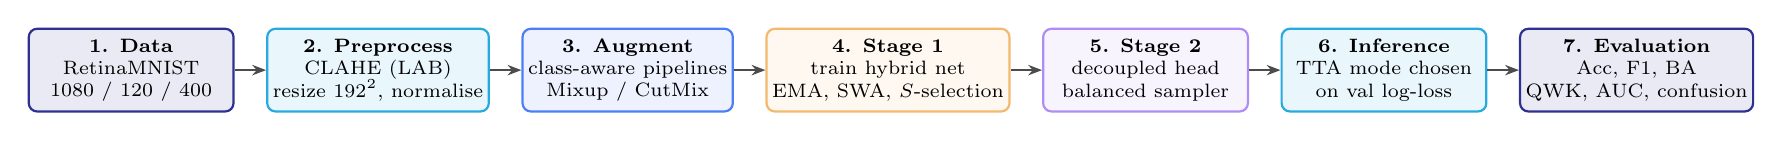
\begin{tikzpicture}[
  st/.style={draw=#1,fill=#1!10,rounded corners=3pt,thick,minimum width=2.6cm,minimum height=1.05cm,align=center,font=\scriptsize,inner sep=2pt},
  arr/.style={-{Stealth[length=5pt]},thick,black!70}]
\node[st=ind] (s1) {\textbf{1. Data}\\RetinaMNIST\\1080 / 120 / 400};
\node[st=cyn,right=0.4cm of s1] (s2) {\textbf{2. Preprocess}\\CLAHE (LAB)\\resize 192$^2$, normalise};
\node[st=blu,right=0.4cm of s2] (s3) {\textbf{3. Augment}\\class-aware pipelines\\Mixup / CutMix};
\node[st=org,right=0.4cm of s3] (s4) {\textbf{4. Stage 1}\\train hybrid net\\EMA, SWA, $S$-selection};
\node[st=pur,right=0.4cm of s4] (s5) {\textbf{5. Stage 2}\\decoupled head\\balanced sampler};
\node[st=cyn,right=0.4cm of s5] (s6) {\textbf{6. Inference}\\TTA mode chosen\\on val log-loss};
\node[st=ind,right=0.4cm of s6] (s7) {\textbf{7. Evaluation}\\Acc, F1, BA\\QWK, AUC, confusion};
\foreach \a/\b in {s1/s2,s2/s3,s3/s4,s4/s5,s5/s6,s6/s7} \draw[arr] (\a) -- (\b);
\end{tikzpicture}}
\caption{End-to-end workflow of the proposed system.}\label{fig:flow}
\end{figure*}

Figure~\ref{fig:flow} shows the end-to-end workflow and Fig.~\ref{fig:arch} the network.
Given an image $x\in\mathbb{R}^{3\times192\times192}$, three parts operate in sequence: a CNN for local features, a Transformer for global context and a classifier head.

\begin{figure*}[t]
\centering
\resizebox{\textwidth}{!}{%
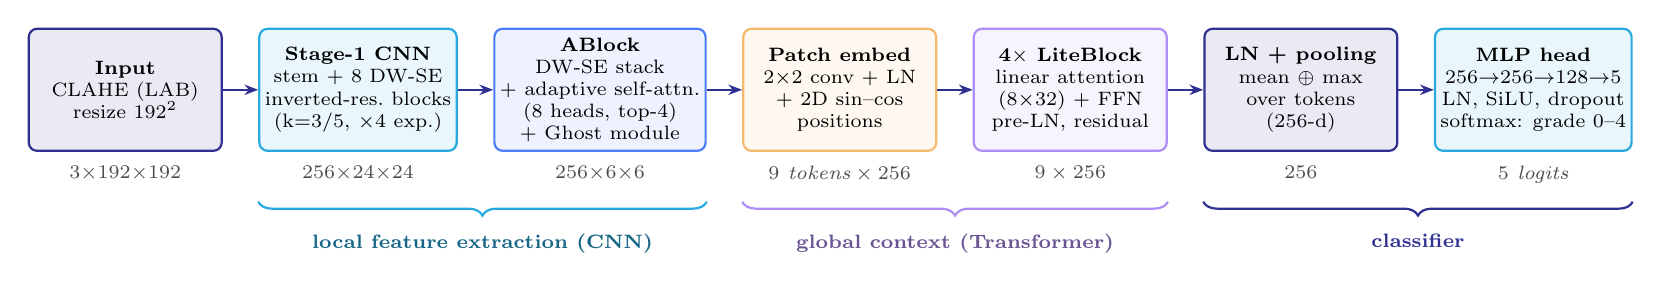
\begin{tikzpicture}[
  blk/.style={draw=#1,fill=#1!10,rounded corners=3pt,thick,minimum width=2.45cm,minimum height=1.55cm,align=center,font=\scriptsize,inner sep=2pt},
  arr/.style={-{Stealth[length=5pt]},thick,ind},
  dim/.style={font=\scriptsize\itshape,text=black!70,align=center}]
\node[blk=ind] (a) {\textbf{Input}\\CLAHE (LAB)\\resize $192^2$};
\node[blk=cyn,right=0.45cm of a] (b) {\textbf{Stage-1 CNN}\\stem + 8 DW-SE\\inverted-res.\ blocks\\(k=3/5, $\times4$ exp.)};
\node[blk=blu,right=0.45cm of b] (c) {\textbf{ABlock}\\DW-SE stack\\+ adaptive self-attn.\\(8 heads, top-4)\\+ Ghost module};
\node[blk=org,right=0.45cm of c] (d) {\textbf{Patch embed}\\$2{\times}2$ conv + LN\\+ 2D sin--cos\\positions};
\node[blk=pur,right=0.45cm of d] (e) {\textbf{4$\times$ LiteBlock}\\linear attention\\(8$\times$32) + FFN\\pre-LN, residual};
\node[blk=ind,right=0.45cm of e] (f) {\textbf{LN + pooling}\\mean $\oplus$ max\\over tokens\\(256-d)};
\node[blk=cyn,right=0.45cm of f] (g) {\textbf{MLP head}\\256$\to$256$\to$128$\to$5\\LN, SiLU, dropout\\softmax: grade 0--4};
\foreach \s/\t in {a/b,b/c,c/d,d/e,e/f,f/g} \draw[arr] (\s) -- (\t);
\node[dim,below=0.05cm of a] {$3{\times}192{\times}192$};
\node[dim,below=0.05cm of b] {$256{\times}24{\times}24$};
\node[dim,below=0.05cm of c] {$256{\times}6{\times}6$};
\node[dim,below=0.05cm of d] {$9\ \text{tokens}\times256$};
\node[dim,below=0.05cm of e] {$9\times256$};
\node[dim,below=0.05cm of f] {$256$};
\node[dim,below=0.05cm of g] {$5$ logits};
\draw[decorate,decoration={brace,amplitude=5pt,raise=18pt,mirror},thick,cyn] (b.south west) -- (c.south east) node[midway,below=26pt,font=\scriptsize\bfseries,text=cyn!60!black] {local feature extraction (CNN)};
\draw[decorate,decoration={brace,amplitude=5pt,raise=18pt,mirror},thick,pur] (d.south west) -- (e.south east) node[midway,below=26pt,font=\scriptsize\bfseries,text=pur!60!black] {global context (Transformer)};
\draw[decorate,decoration={brace,amplitude=5pt,raise=18pt,mirror},thick,ind] (f.south west) -- (g.south east) node[midway,below=26pt,font=\scriptsize\bfseries,text=ind] {classifier};
\end{tikzpicture}}
\caption{Architecture of the proposed hybrid network (7.99\,M parameters). Tensor sizes are shown below each block.}\label{fig:arch}
\end{figure*}

\subsection{Local feature extractor}
The stem is a $3{\times}3$ stride-2 convolution (64 channels). It is followed by eight inverted-residual blocks with squeeze-and-excitation~\cite{senet,mobilenetv2} (expansion 4, depthwise kernels 3 or 5, SiLU activations), arranged in three stages of 64, 128 and 256 channels with stride-2 down-sampling between stages, and a depthwise $3{\times}3$ refinement convolution. The output is a $256{\times}24{\times}24$ feature map. Channel dropout (2D, $p{=}0.05$) regularises this map.

\subsection{Adaptive self-attention block (ABlock)}
The ABlock applies a second DW-SE stack (256$\to$64$\to$256 channels, down-sampling to $6{\times}6$), then an \emph{adaptive self-attention} layer, a Ghost module~\cite{ghostnet} and a residual connection with batch normalisation. The attention layer extends standard multi-head attention with: a depthwise positional convolution added to the input; LayerNorm on queries and keys; a learnable temperature per head; ``talking-heads'' mixing matrices before and after the softmax; and a \emph{head gate} that predicts a softmax distribution over the 8 heads from globally pooled features and keeps only the top-$k{=}4$ heads, weighted by their gate probabilities. The output is $x+\gamma\,\mathrm{Proj}(\cdot)+\alpha\,\mathrm{Local}(x)$ with learnable scalars $\gamma$ and $\alpha$ (initialised to 0.5 and 0.25) and a depthwise-separable local branch.

\subsection{Linear-attention Transformer and head}
The $256{\times}6{\times}6$ map is split into $2{\times}2$ patches (9 tokens, 256-d, LayerNorm) and a 2D sinusoidal position embedding is added. Four \emph{LiteBlocks} follow, each with a pre-LN linear-attention layer and a feed-forward network (expansion 2, SiLU, dropout). Linear attention uses the feature map $\phi(\cdot)=\mathrm{elu}(\cdot)+1$:
\begin{equation}
\mathrm{Attn}(Q,K,V)=\frac{\phi(Q)\,\bigl(\phi(K)^{\top}V\bigr)}{\phi(Q)\,\sum_j\phi(K_j)^{\top}},
\end{equation}
which costs $\mathcal{O}(N d^2)$ instead of $\mathcal{O}(N^2 d)$; the output is scaled by 0.5. With only $N{=}9$ tokens the saving is small at this resolution, but the layer keeps the design scalable to larger inputs. After a final LayerNorm, token features are fused by summing mean and max pooling, and a three-layer MLP head (256$\to$256$\to$128$\to$5, dropout 0.2/0.15/0.1) outputs the grade logits. All dropout rates are scaled by 0.5 in our configuration.

%------------------------------------------------------------------
\section{Training Strategy}\label{sec:train}
\textbf{Class-balanced weights.} For class $c$ with $n_c$ training images, $w_c\propto(1-\beta)/(1-\beta^{n_c})$ with $\beta{=}0.999$~\cite{cbloss}. The ratio $w_{\max}/w_{\min}$ is capped at 3 so that no rare class dominates, grade~2 receives an additional factor 1.25 (it lies between two neighbours and is often absorbed by grade~1), and weights are normalised to mean 1. The resulting weights are $(0.425, 1.275, 1.098, 0.927, 1.275)$.

\textbf{Ordinal focal loss.} For a sample with label $y$, the target distribution is $q_y=1-\varepsilon$ and $q_c=\varepsilon\,e^{-|c-y|}/\sum_{k\ne y}e^{-|k-y|}$ for $c\ne y$, with $\varepsilon{=}0.07$, so probability mass leaks mostly to neighbouring grades. The loss is
\begin{equation}
\mathcal{L}=w_y\,(1-p_y)^{\gamma}\Bigl(-\textstyle\sum_{c}q_c\log p_c\Bigr),\quad \gamma=1.5 .
\label{eq:loss}
\end{equation}
For Mixup/CutMix batches the loss is the $\lambda$-weighted sum over the two label sets.

\textbf{Optimisation and averaging.} We use AdamW~\cite{adamw} (learning rate $2{\times}10^{-4}$, weight decay $10^{-3}$, no decay on biases and normalisation parameters), a 5-epoch linear warm-up followed by cosine decay to $10^{-6}$, batch size 32, mixed precision, gradient clipping at 3.0, at most 150 epochs and early stopping with patience 35. An exponential moving average (EMA, decay 0.99 with a warm-up ramp) of the weights is used for validation; SWA~\cite{swa} accumulates weights from epoch 97 (65\% of training) and re-estimates batch-norm statistics.

\textbf{Checkpoint selection.} Because the validation split is tiny, we select checkpoints with a smoothed composite score
\begin{equation}
\begin{split}S={}&(1-\lambda)\bigl(0.45\,\mathrm{F1}+0.45\,\mathrm{BA}\\&+0.05\,\mathrm{Acc}+0.05\,\mathrm{AUC}\bigr)+\lambda\,\mathrm{QWK}\end{split},
\end{equation}
with $\lambda{=}0.12$, averaged over the last five epochs. A low QWK weight prevents the selection from favouring models that hedge toward the crowded middle grades. The EMA-best and SWA checkpoints are compared on $S$ and the better one is kept.

\textbf{Decoupled head fine-tuning (stage 2).} Following~\cite{decouple}, the backbone is frozen and only the classifier head is trained for 10 epochs (AdamW, lr $5{\times}10^{-5}$) on a class-balanced sampler; the best epoch by $S$ is kept, otherwise stage-1 weights are restored.

\textbf{Test-time augmentation (TTA).} Candidate modes are none, horizontal flip (2 views), flips (4 views) and the dihedral group D4 (8 views). The mode with the lowest validation log-loss is used for the test set.

\begin{algorithm}[t]
\small
\DontPrintSemicolon
\SetAlgoLined
\caption{Two-stage training and inference}\label{alg:train}
Compute class weights $w$; build loss $\mathcal{L}$ (Eq.~\ref{eq:loss}); init EMA, SWA\;
\For{epoch $=1$ \KwTo $150$}{
  set $p_s$ and Mixup/CutMix probability from the 3-stage schedule\;
  \ForEach{batch}{apply class-aware augmentation and optional Mixup/CutMix; forward (AMP); minimise $\mathcal{L}$ with AdamW, clip gradients; update EMA}
  evaluate EMA weights on validation; update $S$ (5-epoch mean); keep best; early-stop if no gain for 35 epochs\;
  \lIf{epoch $\ge 97$}{update SWA}
}
Keep EMA-best or SWA, whichever has the higher $S$\;
Freeze backbone; fine-tune head 10 epochs on balanced sampler; keep best by $S$\;
Choose TTA mode by validation log-loss; predict the test set\;
\end{algorithm}

\textbf{Reproducibility.} All random generators are seeded (seed 42); cuDNN is set to deterministic mode with benchmarking disabled, and the shuffling data loader has its own seeded generator.

%------------------------------------------------------------------
\section{Experimental Setup}\label{sec:exp}
Table~\ref{tab:hp} lists the configuration. The model has 7.99\,M parameters and an epoch takes about 17\,s on a single CUDA GPU with mixed precision. Training stopped by early stopping at epoch 114; the best EMA checkpoint was from epoch 79. Metrics are accuracy, macro precision/recall/F1, balanced accuracy (BA), quadratic weighted kappa (QWK) and macro one-vs-rest AUC. The framework is PyTorch~\cite{pytorch}.

\textbf{Evaluation protocol.} The official RetinaMNIST split is used without modification. The training split is used for fitting, the validation split for checkpoint selection (score $S$), the choice between EMA and SWA weights, and the choice of TTA mode, and the test split for the final report. All test-set numbers in this paper come from one run with seed 42.

\textbf{Computational cost.} The network has 7.99\,M parameters, about 68\% of the roughly 11.7\,M of a standard ResNet-18 and about 31\% of the 25.6\,M of ResNet-50 in their ImageNet configurations, and one training epoch takes about 17\,s on a single GPU. The whole schedule (114 epochs plus 10 head-tuning epochs) therefore runs in well under an hour, which makes repeated seeds and cross-validation affordable for future work.

\textbf{Metrics.} With $C{=}5$ grades, macro precision, recall and F1 average the per-class values; balanced accuracy is the mean per-class recall. QWK is $\kappa=1-\sum_{ij}w_{ij}O_{ij}/\sum_{ij}w_{ij}E_{ij}$ with $w_{ij}=(i-j)^2/(C-1)^2$, where $O$ is the observed confusion matrix and $E$ the expected one under independence; it penalises errors in proportion to their grade distance and is therefore the most clinically meaningful ordinal metric here. AUC is the macro-average of one-vs-rest areas under the ROC curve computed from the softmax probabilities.

\begin{table}[t]
\centering\footnotesize
\caption{Main hyper-parameters.}\label{tab:hp}
\begin{tabular}{p{2.55cm}p{4.85cm}}
\toprule
Parameter & Value\\
\midrule
Input / split & $192{\times}192$ (CLAHE); 1080/120/400\\
Optimiser & AdamW, wd $10^{-3}$, batch 32\\
Learning rate & $2{\times}10^{-4}$; warm-up 5, cosine to $10^{-6}$\\
Epochs & 150 max, patience 35 (stopped at 114)\\
Loss & ordinal focal, $\gamma{=}1.5$, $\varepsilon{=}0.07$\\
Class weights & CB $\beta{=}0.999$, ratio cap 3, G2$\times$1.25\\
Mixup/CutMix & $\alpha{=}0.4$, $p\in\{0,0.15,0.25\}$\\
Averaging & EMA 0.99; SWA from epoch 97\\
Stage 2 & head only, balanced sampler, 10 ep.\\
Model & base 64, embed 256, depth 4, 7.99\,M\\
\bottomrule
\end{tabular}
\end{table}

%------------------------------------------------------------------
\section{Results and Analysis}
\textbf{Overall performance.} On the held-out test set the final system (stage-1 EMA checkpoint, decoupled head, horizontal-flip TTA) obtains accuracy 0.580, macro-precision 0.524, macro-recall 0.521, macro-F1 0.514, BA 0.521, QWK 0.728 and AUC 0.832 (test loss 1.074). The corresponding validation numbers are 0.625, 0.564, 0.620, 0.568, 0.620, 0.707 and 0.831. The gap between validation and test macro-F1 (0.568 vs.\ 0.514) is plausible given the 120-image validation set.


\begin{table}[t]
\centering\footnotesize
\caption{Final validation and test metrics of the selected system (single run, seed 42).}\label{tab:final}
\begin{tabular}{lcc}
\toprule
Metric & Validation (120) & Test (400)\\
\midrule
Accuracy & 0.625 & \textbf{0.580}\\
Precision (macro) & 0.564 & \textbf{0.524}\\
Recall (macro) & 0.620 & \textbf{0.521}\\
F1-score (macro) & 0.568 & \textbf{0.514}\\
Balanced accuracy & 0.620 & \textbf{0.521}\\
QWK & 0.707 & \textbf{0.728}\\
AUC (OvR, macro) & 0.831 & \textbf{0.832}\\
Cross-entropy loss & -- & \textbf{1.074}\\
\bottomrule
\end{tabular}
\end{table}

Table~\ref{tab:final} summarises the final accuracy, precision, recall and F1-score on both splits; per-class values follow in Table~\ref{tab:cls}.

\begin{figure*}[t]
\centering
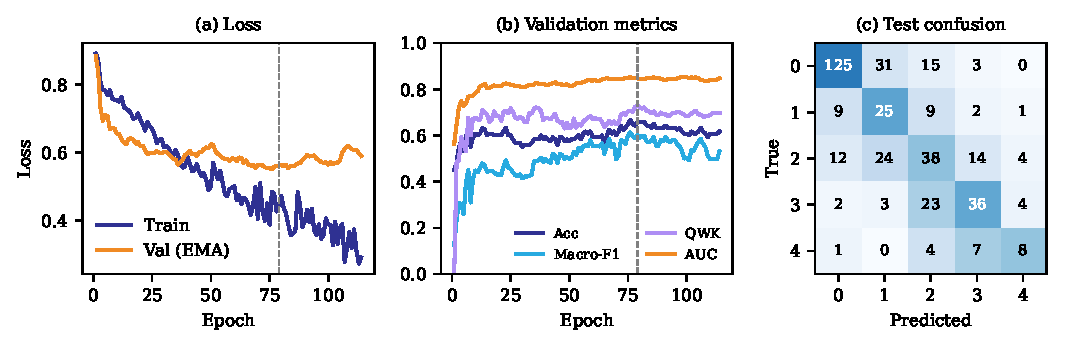
\includegraphics[width=\textwidth]{results.pdf}
\caption{(a) Training and validation loss (EMA weights for validation); the dashed line marks the selected epoch 79. (b) Validation metrics per epoch. (c) Confusion matrix on the test set (counts; shading shows the row-normalised share).}\label{fig:res}
\end{figure*}

\begin{table}[t]
\centering\footnotesize
\caption{Per-class results on the test set.}\label{tab:cls}
\begin{tabular}{lcccc}
\toprule
Grade & Precision & Recall & F1 & Support\\
\midrule
0 & 0.839 & 0.718 & 0.774 & 174\\
1 & 0.301 & 0.543 & 0.388 & 46\\
2 & 0.427 & 0.413 & 0.420 & 92\\
3 & 0.581 & 0.529 & 0.554 & 68\\
4 & 0.471 & 0.400 & 0.432 & 20\\
\midrule
Macro avg. & 0.524 & 0.521 & 0.514 & 400\\
Weighted avg. & 0.620 & 0.580 & 0.594 & 400\\
\bottomrule
\end{tabular}
\end{table}

\textbf{Per-class behaviour.} Table~\ref{tab:cls} shows that the majority grade~0 is recognised best (F1 0.774). Grade~1 reaches a recall of 0.543 despite only 128 training images, but its precision is low (0.301) because 31 of the 174 grade-0 images are assigned to grade~1, a side effect of the class-balanced weighting. Grades~2 and~3 are confused with their neighbours (24 grade-2 images predicted as grade~1; 23 grade-3 images predicted as grade~2). Grade~4 has only 20 test images, so its estimates are very uncertain.

\textbf{Ordinal structure of the errors.} Of the 168 misclassified test images, 121 (72.0\%) are one grade away from the truth, 40 (23.8\%) two grades away, and only 7 (4.2\%) three or four grades away (Fig.~\ref{fig:res}c). This explains why QWK (0.728) and AUC (0.832) are comparatively high relative to accuracy (0.580): the model captures severity ordering even when the exact grade is wrong.

\textbf{Row-wise error analysis.} Reading the confusion matrix (Fig.~\ref{fig:res}c) by true grade gives per-class recalls of 125/174 (grade~0), 25/46 (grade~1), 38/92 (grade~2), 36/68 (grade~3) and 8/20 (grade~4). The largest single error mass is grade~0 predicted as grade~1 (31 images, 17.8\% of grade~0). Grade~2 is the most diffuse class: 24 of its images go down to grade~1 and 14 go up to grade~3. Grade~4 errors are concentrated on grade~3 (7 of 12 misclassified images). No grade-4 image is predicted as grade~1, and only one is predicted as grade~0.

\textbf{Referable-DR view.} Collapsing the five grades into non-referable (grades 0--1) and referable (grades 2--4), a common screening split, the same confusion matrix gives a sensitivity of 138/180 (0.767), a specificity of 190/220 (0.864) and a binary accuracy of 0.820. This derived figure was not a training objective, and it is computed on the same single test run, so it carries the same uncertainty as the other numbers.

\begin{table}[t]
\centering\footnotesize
\caption{Comparison with the published MedMNIST~v2 RetinaMNIST baselines~\cite{medmnistv2} (test set).}\label{tab:cmp}
\begin{tabular}{lcc}
\toprule
Method (input size) & AUC & ACC\\
\midrule
ResNet-18 (28)       & 0.717 & 0.524\\
ResNet-18 (224)      & 0.710 & 0.493\\
ResNet-50 (28)       & 0.726 & 0.528\\
Google AutoML Vision & 0.750 & 0.531\\
\midrule
\textbf{Ours (7.99\,M, 192, from scratch)} & \textbf{0.832} & \textbf{0.580}\\
\bottomrule
\end{tabular}
\end{table}

\textbf{Comparison with MedMNIST v2.} Table~\ref{tab:cmp} places the system next to the benchmark baselines reported with MedMNIST~v2~\cite{medmnistv2}. The proposed network exceeds the strongest listed baseline (Google AutoML Vision) by 4.9 points of accuracy (0.580 vs.\ 0.531) and by 0.082 AUC (0.832 vs.\ 0.750), and exceeds the ResNet baselines by 5.2--8.7 accuracy points. These numbers should be read with care: the baselines were trained by the benchmark authors with a different, untuned protocol and at 28 or 224 pixels, whereas our system uses 192-pixel inputs, CLAHE and a recipe that was tuned for this dataset, partly while observing test-set behaviour (see Section~\ref{sec:disc}). The comparison therefore shows that the proposed system is competitive on this benchmark, not that each architectural component is responsible for the gain.

\textbf{Statistical uncertainty.} With 400 test images, the normal-approximation 95\% confidence interval for an accuracy of 0.580 is about $\pm0.048$ (0.532--0.628), which treats test images as independent and ignores selection effects from model development. The 4.9-point accuracy margin over the strongest baseline is therefore of the same size as the sampling uncertainty of a single test accuracy, whereas the 0.082 AUC margin is larger. Repeated seeds or cross-validation are needed before the accuracy ranking can be called reliable.

\begin{table}[t]
\centering\footnotesize
\caption{Stage-wise validation results. ``LL'' is validation log-loss (TTA candidates only); the selected row is in bold.}\label{tab:stage}
\setlength{\tabcolsep}{3.6pt}
\begin{tabular}{lccccc}
\toprule
Configuration & Acc & F1 & BA & QWK & AUC\\
\midrule
EMA-best (epoch 79) & .658 & .601 & .649 & .729 & .848\\
SWA (18 updates) & .625 & .561 & .588 & .690 & .848\\
+ Decoupled head (LL 1.116) & .658 & .599 & .664 & .722 & .835\\
\textbf{+ H-flip TTA (LL 1.109)} & \textbf{.625} & \textbf{.568} & \textbf{.620} & \textbf{.707} & \textbf{.831}\\
+ 4-view flip TTA (LL 1.124) & .592 & .533 & .582 & .704 & .828\\
+ D4 TTA (LL 1.149) & .533 & .431 & .441 & .648 & .816\\
\bottomrule
\end{tabular}
\end{table}

\textbf{Stage-wise analysis.} Table~\ref{tab:stage} traces the pipeline on the validation set. SWA did not beat the EMA checkpoint on $S$ (0.602 vs.\ 0.644) and was discarded. Decoupled head fine-tuning improved the selection score marginally (0.649$\to$0.653) at the cost of a small AUC drop. Horizontal-flip TTA obtained the lowest validation log-loss and was selected, although it lowered validation accuracy; richer TTA (4 and 8 views) clearly hurt. This suggests that vertical flips and rotations alter fundus appearance (e.g.\ optic-disc position relative to the macula) in ways the model was not trained to be invariant to, and also illustrates that a log-loss criterion and an accuracy criterion can disagree on a 120-image set.

%------------------------------------------------------------------
\section{Discussion and Limitations}\label{sec:disc}
The system trades peak accuracy for a small model (7.99\,M parameters) and a stable training recipe, and its errors are mostly between adjacent grades, which is clinically more benign than distant confusions. Nevertheless, an accuracy of 0.580 is modest and should not be read as clinical-grade performance. We highlight the following limitations.
\begin{itemize}
\item \textbf{Small data and noisy selection.} With 1,080 training and 120 validation images, checkpoint and TTA selection are noisy; test class~4 has only 20 images.
\item \textbf{Single run.} Only seed~42 is reported; no repeated runs, cross-validation or confidence intervals are available, so small differences should not be over-interpreted.
\item \textbf{No ablation; baselines not re-run.} We do not report ablations of individual components, and the MedMNIST~v2 baselines in Table~\ref{tab:cmp} are the published numbers rather than models we re-trained under our protocol (they also use different input resolutions); the contribution of each ingredient is therefore not isolated. This is left to future work.
\item \textbf{Possible optimistic bias.} During development some settings (for example the extra weight on grade~2 and the label-smoothing amount) were adjusted after inspecting error patterns, including an earlier test-set confusion matrix. Test numbers may therefore be slightly optimistic; a cleaner protocol would tune only on validation data or use cross-validation.
\item \textbf{Precision--recall trade-off.} Class-balanced weighting raises grade-1 recall to 0.543 but lowers its precision to 0.301, since 31 grade-0 images are pulled into grade~1. Whether this trade is desirable depends on the screening policy: a false alarm costs a re-check, a missed case costs more.
\item \textbf{Illustrative scope.} The images are low-resolution benchmark versions of fundus photographs, and no external dataset or clinical validation was performed.
\item \textbf{Not for clinical use.} The model is a research prototype; any screening use would need prospective validation and human oversight.
\end{itemize}

\textbf{Directions for future work.} Repeated seeds and $k$-fold cross-validation would give confidence intervals and remove the dependence on a 120-image validation set. Component-wise ablations and baselines re-trained under the same recipe would show which ingredients matter and make the comparison fair.

%------------------------------------------------------------------
\section{Conclusion}
We presented a reproducible system for five-grade diabetic retinopathy classification on RetinaMNIST, built around a 7.99\,M-parameter hybrid of a depthwise SE-CNN, adaptive self-attention and a linear-attention Transformer, trained with an imbalance- and ordinality-aware recipe. It achieves 58.0\% accuracy, 0.728 QWK and 0.832 AUC on the test set, with most errors between adjacent grades, ahead of the published MedMNIST~v2 baselines (best 0.531 accuracy, 0.750 AUC). Future work includes multi-seed and cross-validated evaluation, re-trained baselines and ablation studies, an ordinal-regression head, self-supervised pre-training on unlabelled fundus images and higher-resolution inputs.

\section*{Acknowledgment}
The author thanks the BUBT CV Competition organisers for the dataset and event, the MedMNIST team for releasing RetinaMNIST, and the supervisor, Md.\ Darun Nayeem, for guidance.

%------------------------------------------------------------------
\begingroup
\footnotesize
\setlength{\itemsep}{0pt}
\begin{thebibliography}{99}\setlength{\itemsep}{3pt}\setlength{\parsep}{0pt}
\bibitem{gulshan} V.~Gulshan \emph{et al.}, ``Development and validation of a deep learning algorithm for detection of diabetic retinopathy in retinal fundus photographs,'' \emph{JAMA}, vol.~316, no.~22, pp.~2402--2410, 2016.
\bibitem{medmnistv2} J.~Yang \emph{et al.}, ``MedMNIST v2 -- A large-scale lightweight benchmark for 2D and 3D biomedical image classification,'' \emph{Scientific Data}, vol.~10, art.~41, 2023.
\bibitem{vaswani} A.~Vaswani \emph{et al.}, ``Attention is all you need,'' in \emph{Proc.\ NeurIPS}, 2017, pp.~5998--6008.
\bibitem{vit} A.~Dosovitskiy \emph{et al.}, ``An image is worth 16x16 words: Transformers for image recognition at scale,'' in \emph{Proc.\ ICLR}, 2021.
\bibitem{deepdrid} R.~Liu \emph{et al.}, ``DeepDRiD: Diabetic retinopathy---grading and image quality estimation challenge,'' \emph{Patterns}, vol.~3, no.~6, 2022.
\bibitem{resnet} K.~He, X.~Zhang, S.~Ren, and J.~Sun, ``Deep residual learning for image recognition,'' in \emph{Proc.\ CVPR}, 2016, pp.~770--778.
\bibitem{efficientnet} M.~Tan and Q.~V.~Le, ``EfficientNet: Rethinking model scaling for convolutional neural networks,'' in \emph{Proc.\ ICML}, 2019, pp.~6105--6114.
\bibitem{senet} J.~Hu, L.~Shen, and G.~Sun, ``Squeeze-and-excitation networks,'' in \emph{Proc.\ CVPR}, 2018, pp.~7132--7141.
\bibitem{mobilenetv2} M.~Sandler \emph{et al.}, ``MobileNetV2: Inverted residuals and linear bottlenecks,'' in \emph{Proc.\ CVPR}, 2018, pp.~4510--4520.
\bibitem{ghostnet} K.~Han \emph{et al.}, ``GhostNet: More features from cheap operations,'' in \emph{Proc.\ CVPR}, 2020, pp.~1580--1589.
\bibitem{linattn} A.~Katharopoulos \emph{et al.}, ``Transformers are RNNs: Fast autoregressive Transformers with linear attention,'' in \emph{Proc.\ ICML}, 2020, pp.~5156--5165.
\bibitem{mobilevit} S.~Mehta and M.~Rastegari, ``MobileViT: Light-weight, general-purpose, and mobile-friendly vision transformer,'' in \emph{Proc.\ ICLR}, 2022.
\bibitem{cbloss} Y.~Cui \emph{et al.}, ``Class-balanced loss based on effective number of samples,'' in \emph{Proc.\ CVPR}, 2019, pp.~9268--9277.
\bibitem{focal} T.-Y.~Lin \emph{et al.}, ``Focal loss for dense object detection,'' in \emph{Proc.\ ICCV}, 2017, pp.~2980--2988.
\bibitem{mixup} H.~Zhang \emph{et al.}, ``mixup: Beyond empirical risk minimization,'' in \emph{Proc.\ ICLR}, 2018.
\bibitem{cutmix} S.~Yun \emph{et al.}, ``CutMix: Regularization strategy to train strong classifiers with localizable features,'' in \emph{Proc.\ ICCV}, 2019, pp.~6023--6032.
\bibitem{decouple} B.~Kang \emph{et al.}, ``Decoupling representation and classifier for long-tailed recognition,'' in \emph{Proc.\ ICLR}, 2020.
\bibitem{swa} P.~Izmailov \emph{et al.}, ``Averaging weights leads to wider optima and better generalization,'' in \emph{Proc.\ UAI}, 2018.
\bibitem{cohen} J.~Cohen, ``Weighted kappa: Nominal scale agreement with provision for scaled disagreement or partial credit,'' \emph{Psychol.\ Bull.}, vol.~70, no.~4, pp.~213--220, 1968.
\bibitem{clahe} K.~Zuiderveld, ``Contrast limited adaptive histogram equalization,'' in \emph{Graphics Gems IV}, Academic Press, 1994, pp.~474--485.
\bibitem{adamw} I.~Loshchilov and F.~Hutter, ``Decoupled weight decay regularization,'' in \emph{Proc.\ ICLR}, 2019.
\bibitem{pytorch} A.~Paszke \emph{et al.}, ``PyTorch: An imperative style, high-performance deep learning library,'' in \emph{Proc.\ NeurIPS}, 2019.
\end{thebibliography}
\endgroup

\end{document}
